\documentclass{standalone}
\usepackage{tikz}
\usepackage{ctex,siunitx}
\setCJKmainfont{Noto Serif CJK SC}
\usepackage{tkz-euclide}
\usepackage{amsmath}
\usetikzlibrary{patterns, calc}
\usetikzlibrary {decorations.pathmorphing, decorations.pathreplacing, decorations.shapes,}

\begin{document}
\small
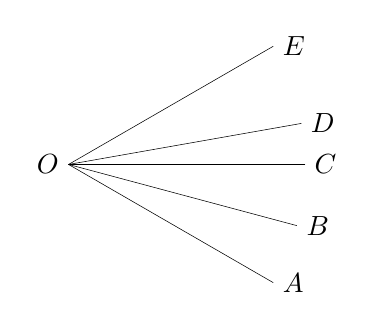
\begin{tikzpicture}[>=stealth,scale=1.0]
  \tkzSetUpPoint[fill=black]
  % \useasboundingbox(-1,-0.75)rectangle(3.7,1.4);
  \tkzDefPoints{0/0/O}
  \tkzDefPoint(-30:3){A}
  \tkzDefPoint(-15:3){B}
  \tkzDefPoint(0:3){C}
  \tkzDefPoint(10:3){D}
  \tkzDefPoint(30:3){E}
  \tkzDrawSegments(A,O B,O C,O D,O E,O)
  \tkzLabelPoints[right](A,B,C,D,E)	  
  \tkzLabelPoints[left](O)	
\end{tikzpicture}
\end{document}